\begin{document}

\section{Bakgrund: artificiell intelligens och djupinlärning}
\label{sec:DeepBack}

Artificiell intelligens är ett samlingsbegrepp för metoder som automatiserar intellektuella uppgifter som vanligen utförs av människor \cite{Chollet}. Bland dessa metoder ingår maskin- och djupinlärning. I detta kapitel presenteras den grundläggande teorin bakom djupinlärning, och därefter hur djupinlärning kan kombineras med och analyseras av statistiska metoder. 

Djupinlärning är ett underfält till maskininlärning. Skillnaden mellan maskininlärning och klassisk programmering finns i vilken typ av problem de används till. Det klassiska programmeringsproblemet kan definieras som att utifrån indata $\mathbb{X}$ generera resultat $\mathbb{Y}$, genom att behandla indatan efter en fördefinierad sekvens av regler \cite{JavaGroundUp}. Det generella maskininlärningsproblemet kan definieras som att utifrån en indatamängd $\mathbb{X}$ finna en sannolikhetsfördelning $q\left(\mathbb{Y}|\mathbb{X}\right)$ som optimalt approximerar den sanna fördelningen $p\left(\mathbb{Y}|\mathbb{X}\right)$ \cite{variation}. Förenklat är målet att utifrån given data $\mathbb{X}$ finna en modell $q$ som sedan kan användas för att generera förutsägelser som stämmer väl överens med verkliga resultat $p$. I ordet maskininlärning kommer ''inlärningen'' från processen att finna modellen $q$. Processen kallas att träna ett maskininlärningssystem.
\begin{figure}[hbtp]
    \centering
    \resizebox {0.7\textwidth} {!} {
        \definecolor{input_node}{RGB}{171,171,154}
\definecolor{dense_node}{RGB}{196,225,144}
\definecolor{dropout_node}{RGB}{222,222,222}
\definecolor{output_node}{RGB}{171,154,154}
% New colors
\definecolor{klight_green_400}{RGB}{156, 204, 101}

\tikzset{%
  dense neuron/.style={
    circle,
    draw,
    fill=klight_green_400,
    thick,
    minimum size=0.75cm
  },
  dropout neuron/.style={
    circle,
    draw,
    fill=dropout_node,
    thick,
    minimum size=0.75cm
  },
  input neuron/.style={
    circle,
    draw,
    fill=input_node,
    thick,
    minimum size=0.75cm
  },
  output neuron/.style={
    circle,
    draw,
    fill=output_node,
    thick,
    minimum size=0.75cm
  },
  neuron missing/.style={
    draw=none, 
    scale=4,
    fill=none,
    text height=0.333cm,
    execute at begin node=\color{black}$\vdots$
  },
  zoom neuron/.style={
    circle,
    draw,
    fill=klight_green_400,
    opacity=0.3,
    minimum size=1.2cm
  },
  zoom line/.style={
    draw,
    opacity=0.3,
    line width=0.5mm,
    minimum size=1cm
  },
  z_connect line/.style={
    draw,
    line width=0.4mm,
    minimum size=1cm
  },
  highlight neuron/.style={
    circle,
    draw,
    fill=klight_green_400,
    minimum size=1.2cm
  },
  highlight line/.style={
    draw,
    opacity=1,
    line width=0.5mm,
    minimum size=1cm
  },
}

\begin{tikzpicture}[x=1.5cm, y=1.5cm, >=stealth]
\foreach \m/\l [count=\y] in {1,2,3,missing,4}
  \node [input neuron/.try, neuron \m/.try] (input-\m) at (0,2.5-\y) {};

\foreach \m [count=\y] in {1,missing,2}
  \node [dense neuron/.try, neuron \m/.try ] (hidden1-\m) at (1.5,2-\y*1.25) {};
  \foreach \m [count=\y] in {1,missing,2}
  \node [dense neuron/.try, neuron \m/.try ] (hidden2-\m) at (3,2-\y*1.25) {};

\foreach \m [count=\y] in {1,missing,2}
  \node [input neuron/.try, neuron \m/.try ] (output-\m) at (4.5,1.5-\y) {};

\foreach \l [count=\i] in {1,2,3,n}
  \draw [<-] (input-\i) -- ++(-1,0)
    node [above, midway] {\Large $x_\l$};

\foreach \l [count=\i] in {1,n}
  \draw [->] (output-\i) -- ++(1,0)
    node [above, midway] {\Large  $\hat{y}_\l$};

\foreach \i in {1,...,4}
  \foreach \j in {1,...,2}
    \draw [->] (input-\i) -- (hidden1-\j);
\foreach \i in {1,...,2}
  \foreach \j in {1,...,2}
    \draw [->] (hidden1-\i) -- (hidden2-\j);

\foreach \i in {1,...,2}
  \foreach \j in {1,...,2}
    \draw [->] (hidden2-\i) -- (output-\j);

\foreach \l [count=\x from 0] in {Indata-, Dolt tätt, Dolt tätt, Utdata-}
  \node [align=center, above] at (\x*1.5,2) {\l \\ lager};
  
  
% draw a box around zoom region

\draw[opacity=0.6, line width=0.3mm, dashed] ($(hidden1-1.north west)+(-0.4,0.4)$) rectangle ($(hidden2-2.south east)+(0.4,-0.4)$)
    node [] (box1) {}
    node (box2) at ($(hidden2-1.north east)+(+0.4,0.4)$)  {};



% ***** zoom

\foreach \m/\l [count=\y] in {1,2}
  \node [zoom neuron/.try, neuron \m/.try] (z_input-\m) at (7.5,5-\y*3-1) {};

\foreach \m [count=\y] in {1, 2}
  \node [zoom neuron/.try, neuron \m/.try ] (z_hidden1-\m) at (10.5,5-\y*3-1) {};


\foreach \l [count=\i] in {1,2}
  \draw [<-, zoom line/.try] (z_input-\i) -- ++(-1,0)
    node [above, midway] {};


\foreach \i in {1,...,2}
  \foreach \j in {1,...,2}
    \draw [->, zoom line/.try] (z_input-\i) -- (z_hidden1-\j);
    
% Mark certain nodes and corresponding lines
\node [highlight neuron/.try, neuron 1/.try ] (highlight-1) at (7.5,5-2*3-1) {\Large $i$};
\node [highlight neuron/.try, neuron 2/.try ] (highlight-2) at (10.5,5-1*3-1) {\Large $j$};
\node at (7.5+0.3,5-2*3-1+0.65) {\Large $x_{i}$};
\draw [->, highlight line/.try] (highlight-1) -- (highlight-2)
    node [] at (9, -0.1) {\Large $w_{ji}$};
\node at (10.5,5-1*3-1+0.65) {\Large $b_j$};
\draw [->, highlight line/.try] (highlight-2) -- ++(1,0)
    node [above, midway] {\Large $u_{j}$};
\draw [->, zoom line/.try] (z_hidden1-2) -- ++(1,0) {};

\draw[opacity=0.6, line width=0.25mm, dashed] ($(z_input-1.north west)+(-0.8,0.6)$) rectangle ($(z_hidden1-2.south east)+(0.8,-0.6)$)
    node (zoom1) at ($(z_input-2.south west)+(-0.8,-0.6)$) {}
    node (zoom2) at ($(z_input-1.north west)+(-0.8,0.6)$)  {};

% **** connect zoom and nn
\begin{scope}[->]
    \path[z_connect line/.try]
        (box1) edge[bend right] node [->, left] {} (zoom1)
        (box2) edge[bend left] node [->, left] {} (zoom2);
\end{scope}
\end{tikzpicture}
    }
    \caption{Ett neuralt nätverk bestående av ett indata-lager, två dolda lager och ett utdata-lager. ${x_1,...,x_n}$ och ${\hat{y_1},...,\hat{y_n}}$ är komponenter till indatan $\mathbb{X}$ respektive utdatan $\mathbb{\hat{Y}}$. Till höger visas en inzoomning... TODO}
    \label{fig:general_NN}
\end{figure}

Vad som utmärker djupinlärning från andra former av maskininlärning är att inom djupinlärning utförs flera transformationer av indatan efter varandra, med förhoppning att varje transformation successivt ger en tydligare representation av indatan. Inom djupinlärning kallas det att nätverket lär sig flera lager av representation \cite{Chollet}. Dessa lager kan representeras med en struktur som kallas för ett \textit{neuralt nätverk}. Ett neuralt nätverk består av flera sammankopplade lager som motsvarar de olika lagren av representation. Det första lagret kallas indatalager, det sista utdatalager och lagren däremellan för dolda lager. Varje lager är i sin tur uppbyggt av flera noder. En nod inom ett lager är sammankopplad med noder i det föregående lagret och i nästa lager, men inte i det egna lagret, se figur \ref{fig:general_NN}. Varje koppling mellan noder är skalad med en vikt $w$. Dessutom är varje nod associerad med ett förskjutningsvärde (eng. \emph{bias}) $b$. Transformationen mellan två noder $i$ och $j$ kan parametriseras av vikter och förskjutningsvärden på följande sätt 

\begin{equation}
    u_j = A_j \left(w_{ji}x_i + b_j\right),
    \label{eq:node_transform}
\end{equation}
där $x_i$ är indata till nod $j$ from nod $i$ och $u_j$ är utdata från nod $j$, se figur \ref{fig:general_NN}. På motsvarande sätt kan den totala transformationen för nod $i$:s lager uttryckas som 

\begin{equation}
    \textbf{u} = A(\textbf{W} \cdot \textbf{x} + \textbf{b}),
    \label{eq:network_transform}
\end{equation}
\noindent där $\textbf{W}$ är en matris innehållande alla vikter mellan alla noder $i$ och $j$, $\textbf{x}$ är indatavektorn till lagret och \textbf{b} är en vektor som innehåller alla noders förskjutningsvärden. $A$ kallas aktitveringsfunktion (eng. \emph{activation function}) \cite{Chollet}. 



Träningen av det neurala nätverket består i att hitta dessa vikter $\textbf{W}$ och förskjutningsvärden $\textbf{b}$ för varje lager som ger den optimala modellen $q$ \cite{Chollet}. Den konventionella metoden för att göra detta är övervakad inlärning (eng. \emph{supvervised learning}). För detta behövs indata $\mathbb{X}$ (eng. \emph{training data}), ihop med måldata $\mathbb{Y}$ (eng. \emph{target data}). Om nätverkets utdata är $\mathbb{\hat{Y}}$ vid indata $\mathbb{X}$ kan en förlustfunktion (eng. \emph{loss function}) $\mathcal{L}\left(\mathbb{\hat{Y}}, \mathbb{Y} \right)$ definieras. Förlustfunktionen ger ett mått på hur väl måldatan $\mathbb{Y}$ överensstämmer med nätverkets utdata $\mathbb{\hat{Y}}$. Förlustfunktionen kan sedan minimeras genom en process som kallas bakåtpropagation (eng. \emph{back propagation}). Då den totala transformationen för nätverket består av enkla tensoroperationer enligt ekvation \eqref{eq:network_transform} med välkänd derivata kan gradienten av förlustfunktionen $\mathcal{L}$ med avseende på nätverkets vikter och förskjutningsvärden beräknas med hjälp av kedjeregeln. Därefter kan vikterna och förskjutningsvärdena uppdateras i motsatt riktning till gradienten, vilket sker successivt från sista till första lagret i nätverket. Denna process utförs av en så kallad optimeringsfunktion, (eng. \emph{optimizer}).

% \begin{figure}[hbtp]
%     \centering
%     \resizebox {0.5\textwidth} {!} {
%         \definecolor{dense_node}{RGB}{196,225,144}
\definecolor{dropout_node}{RGB}{222,222,222}

\tikzset{%
  every neuron/.style={
    circle,
    draw,
    fill=dropout_node,
    opacity=0.3,
    minimum size=1cm
  },
  every line/.style={
    draw,
    opacity=0.3,
    minimum size=1cm
  },
  highlight neuron/.style={
    circle,
    draw,
    fill=dense_node,
    minimum size=1cm
  },
  highligh line/.style={
    draw,
    opacity=1,
    minimum size=1cm
  },
  neuron missing/.style={
    draw=none, 
    fill=none,
    scale=4,
    text height=0.333cm,
    execute at begin node=\color{black}$\vdots$
  },
}


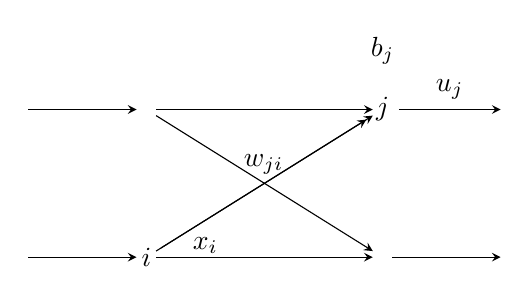
\begin{tikzpicture}[x=1.5cm, y=1.5cm, >=stealth]

\foreach \m/\l [count=\y] in {1,2}
  \node [every neuron/.try, neuron \m/.try] (input-\m) at (0,2.5-\y*1.25) {};

\foreach \m [count=\y] in {1, 2}
  \node [every neuron/.try, neuron \m/.try ] (hidden1-\m) at (2,2.5-\y*1.25) {};

% \foreach \m/\l [count=\y] in {missing,1,2,missing}
%   \node [every neuron/.try, neuron \m/.try] (input-\m) at (0,2.5-\y*1.25) {};

% \foreach \m [count=\y] in {missing, 1, 2, missing}
%   \node [every neuron/.try, neuron \m/.try ] (hidden1-\m) at (2,2.5-\y*1.25) {};
  
% \foreach \m [count=\y] in {missing, 1, 2, missing}
%   \node [every neuron/.try, neuron \m/.try ] (hidden2-\m) at (4,2.5-\y*1.25) {};

% \foreach \m [count=\y] in {1}
%   \node [every neuron/.try, neuron \m/.try ] (output-\m) at (6,-2) {};

\foreach \l [count=\i] in {1,2}
  \draw [<-, every line/.try] (input-\i) -- ++(-1,0)
    node [above, midway] {};

% \foreach \l [count=\i] in {1,n}
%   \node [above] at (hidden-\i.north) {$H_\l$};

% \foreach \l [count=\i] in {j,j+1}
%   \draw [->, every line/.try] (hidden1-\i) -- ++(1,0)
%     node [above, midway] {$u_{\l}$};

\foreach \i in {1,...,2}
  \foreach \j in {1,...,2}
    \draw [->, every line/.try] (input-\i) -- (hidden1-\j);
    
% \foreach \i in {1,...,2}
%   \foreach \j in {1,...,2}
%     \draw [->, every line/.try] (hidden1-\i) -- (hidden2-\j);

% \foreach \i in {1,...,4}
%   \foreach \j in {1}
%     \draw [->, every line/.try] (hidden2-\i) -- (output-\j);

% \foreach \l [count=\x from 0] in {Indata-, Tätt, Tätt, Utdata-}
%   \node [align=center, above] at (\x*2,2) {\l \\ lager};

% Mark certain nodes and corresponding lines
\node [highlight neuron/.try, neuron 1/.try ] (highlight-1) at (0,2.5-2*1.25) {$i$};
\node [highlight neuron/.try, neuron 2/.try ] (highlight-2) at (2,2.5-1*1.25) {$j$};
\node at (2,2.5-1*1.25+0.5) {$b_j$};
\draw [->, highlight line/.try] (highlight-1) -- (highlight-2)
    node [above, midway] {$w_{ji}$};
\node at (0+0.5,2.5-2*1.25+0.1) {$x_{i}$};
\draw [->, highlight line/.try] (highlight-2) -- ++(1,0)
    node [above, midway] {$u_{j}$};
\draw [->, every line/.try] (hidden1-2) -- ++(1,0) {};

\end{tikzpicture}
%     }
%     \caption{En schematisk skiss över hur två noder är kopplade till varandra i ett neuralt nätverk. $x_i$ är utdata från nod $i$, $w_{ij}$ är viktningen av kopplingen mellan nod $i$ och $j$, $b_j$ är förskjutningsvärdet för nod $j$ och $u_j$ dess utdata. Dessa parametrar är relaterade enligt ekvation \eqref{eq:node_transform}.}
%     \label{fig:equation_transform}
% \end{figure}

Ett problem med bakåtpropagation är att nätverkets vikter kan konvergera mot ett lokalt minimum för träningsdatan, men som inte är generellt för problemet. Detta kallas överanpassning. Då neurala nätverk i allmänhet och djupa neurala nätverk i synnerhet har många parametrar i form av deras vikter har de en stor representationsrymd, varför träning nästan alltid resulterar i överanpassning. För att minimera detta problem kommer vi i detta arbete använda oss av tre konventionella metoder: reducera nätverkets storlek, viktregularisation och utsläpp \cite{Chollet}. Reducering av nätverkets storlek minskar representationsrymden, på bekostnad av möjligheten för nätverket att finna mer komplexa mönster i datan. Viktregularisation innebär att nätverkets vikter begränsas till att endast anta låga värden, vilket ger en enklare matematisk modell med lägre risk för överanpassning. Utsläckning innebär att man slumpvis sätter en viss del av indatan till noll vid en viss träningsomgång, vilket ger att motsvarande noder ej bidrar. Detta gör att slumpmässiga mönster i datan inte blir lika tydliga, varför sannolikheten för överanpassning minskar.

Hur väl nätverkets modell generaliserar kan under träning mätas genom att låta nätverket bearbeta ny data. Denna data kallas valideringsdata. För att testa det färdigtränade nätverkets prestanda använder man sig av så kallad testdata. Den tillgängliga datamängden behöver därmed delas in i tre delar: träningsdata, valideringsdata och testdata. Det är viktigt att dessa delar hålls separata, i synnerhet testdatan. Exempelvis om nätverket tränas på delar av testdatan så ger överanpassning en felaktig bild av hur nätverket presterar.
För att sätta nätverkets prestanda i kontext kan man jämföra med en så kallad baslinje (eng. \emph{baseline}) för det aktuella problemet. En baslinje är prestandan som hade erhållits med en annan, oftast enklare, metod än ett neuralt nätverk för det aktuella problemet \cite{Chollet}.

En teknik för att underlätta träningen av de neurala nätverken är genom normalisation av datan. Genom att transformera alla indataparametrar till en $N(0,1)$-fördelning blir viktningen av dem samma, varför nätverket ej behöver hitta hur de olika parametrarna skall viktas. För att undvika kontaminering beräknar man medelvärde $\mu$ och standardavvikelse $\sigma$ på träningsdatan, varefter all data $\mathbb{X}$ normaliseras enligt \cite{Chollet}

\begin{equation}
    \mathbb{X}_{norm} = \frac{\mathbb{X}-\mu}{\sigma}.
    \label{normalization}
\end{equation}

I detta arbete kommer vi ställas mot tre klassiska maskininlärningsproblem: binär klassificering, flerklass-klassificering samt skalär regression. Binär klassificering och flerklass-klassificering innebär att klassificera indata i två respektive flera olika kategorier. Det skalära regressionsproblemet består i att förutsäga ett kontinuerligt värde utifrån indata \cite{Chollet}. För att lösa dessa problem kommer vi använda oss av två speciella typer av djupa neurala nätverk: täta neurala nätverk (eng. \emph{Deep Neural Networks}, DNN) och rekursiva neurala nätverk (eng. \emph{Recurrent Neural Networks}, RNN). Ett RNN har till skillnad från ett DNN ett internt tillstånd baserat på data som det har behandlat tidigare. Ett RNN kan alltså ses som ett återkopplat system där tidigare information sammanvägs med ny, se figur. Detta gör RNN väl lämpade för att behandla sekvenser av data. Specifikt kommer vi använda så kallade långt-korttidsminnesnätverk (eng. \emph{Long short-term memory network}, LSTM), vilka är en speciell implementation av RNN som kan lagra information internt till en senare tidpunkt utöver det interna tillståndet som kännetecknar ett RNN. Detta minimerar risken för att information går förlorad när nätverket arbetar igenom en sekvens.




% Övergripande kan man se ett djupt neuralt nätverk som flera på varandra följande transformationer som omvandlar Ett exempel som Chollet tar upp för att visualisera detta är genom att tänka på hur man själv skulle separera två tillsammans ihopknycklade pappersbitar; genom att göra flera små, enkla rörelser kan till slut veckla ut pappersbitarna, och separarera dem. \cite{Chollet} 
\subsection{Djupa neurala nätverk och osäkerhet}
\label{NN_and_uncert}
Djupa neurala nätverk är utmärkta verktyg för att åstadkomma förutsägelser och klassifieringsalgoritmer. Till exempel som bildigenkänningsalgoritmer, men dessa kan uppvisa opålitligheter vid introduktion av störningar \cite{Elephant}. Problemet kan förklaras av designen av ett kanoniskt klassfieringsproblem eftersom designen tvingar det neurala nätverket att utföra en specifik klassificering. Detta leder till översäkra neurala nätverk \cite{Kendall-Gal}. En möjlig lösning till problemet är att kombinera klassificeringen med en modell för osäkerhet. Detta kan åstadkommas med exempelvis bayesianska neurala nätvärk (eng. Bayesian Neural Networks) eller genom att modifiera förlustfunktionerna för att bygga in en uppskattning av osäkerheter \cite{Kendall-Gal}.

För att underlätta förståelsen av osäkerheter i modellerna introducerar vi begreppen \emph{epistemisk osäkerhet} och \emph{aleatorisk osäkerhet} \cite{Uncert}. Epistemisk osäkerhet kan tolkas som modellosäkerhet medan aleatorisk osäkerhet kan tolkas som en intrinsisk osäkerhet i indatan. Osäkerheterna kan även uttryckas i termer för neurala nätverk. Betrakta ett neuralt nätverk $f^\mathbf{W}$ med vikter och förskjutningsvärden $\mathbf{W}$ och indatamängd $\mathbb{X} = \{\mathbf{x_1},..., \mathbf{x_n}\}$ som avbildar $\mathbf{x_i}$ på förutsägelse $\hat{y}_i = f^\mathbf{W}(\mathbf{x}_i)$ som en uppskattning av utdatamängden $\mathbb{Y} = \{y_1,..., y_n\}$. Det är möjligt utifrån det neurala nätverket som modell att identifiera tre former av osäkerheter i form av aleatorisk indata osäkerhet $\sigma_x$, epistemisk viktosäkerhet $\sigma_W$ och förutsägelse osäkerhet $\sigma_y$.

Det huvudsakliga problemet för att kvantifiera osäkerheter i neurala nätverk är att bestämma en funktion $U$ som utifrån $\sigma_x$ och $\sigma_W$ approximerar osäkerheten i förutsägelse $\sigma_y = U(\sigma_x, \sigma_W)$. Förslagsvis kan $\sigma_W$ uppskattas med bayesiansk djupinlärning (eng. Bayesian Deep Learning) och $\sigma_x$ genom att modifiera vanligt förekommande förlustfunktioner inom djupinlärning \cite{Kendall-Gal}. Emellertid kräver bayesiansk djupinlärning stora mängder beräkningskraft varav approximativa lösningar behöver tillämpas \cite{MC-dropout}. Därav väljer vi för det här arbetet att avgränsa ifrån bayesiansk djupinlärning och epistemisk osäkerhet för att istället fokusera på den aleatoriska osäkerheten i indata. 

I Appendix \ref{app: derivation} visar vi hur aleatorisk osäkerhet $\sigma_x$ kan implementeras i förlustfunktioner och därav uppskattas av neurala nätverk. Under antagande att utdatan är normalfördelad givet indatan är förlustfunktionen
\begin{equation}
    \mathcal{L}_{\mathrm{normal}}(\mathbf{W}) = \exp{\left(-\log \sigma_x^2 \right)} \left\|y - f^\mathbf{W}(\mathbf{x})\right\|_2 + \log \sigma_x^2.
    \label{eq:loss_fcn}
\end{equation}
Speciellt kan det noteras att för konstant $\sigma_x^2$ återfås den kanoniska kvadratiska förlustfunktionen (eng. Mean Squared Error, MSE) $\mathcal{L}_\mathrm{MSE}(\mathbf{W}) = \left\|y - f^\mathbf{W}(\mathbf{x})\right\|_2$. Jämfört med den kvadratiska förlustfunktionen medför den aleatoriska osäkerheten en osäkerhetsattenuationsfaktor $\exp{\left(-\log \sigma_x^2 \right)}$ som minskar bidraget av felet $\left\|y - f^\mathbf{W}(\mathbf{x})\right\|_2$ vid växande osäkerheter $\sigma_x$. Dessutom införs en osäkerhetsterm $\log \sigma_x^2$ som bidrar växande till förlustfunktionen för växande $\sigma_x^2$.

\subsection{Korrelationer för analys av indata}
\label{sec:korre}
Kvaliteten på förutsägelserna $\hat{y}_i = f^\mathbf{W}(\mathbf{x}_i)$ från ett neuralt nätverk påverkas i stor utsträckning av hur väl indatan $\mathbb{X}$ kopplar till måldatan $\mathbb{Y}$. Ett statistisk verktyg för att analysera kopplingen mellan $\mathbb{X}$ och $\mathbb{Y}$ är korrelationskoefficienter. En korrelationskoefficient är ett mått på hur mycket två variabler korrelerar linjärt med varandra. Den vanligaste varianten är Pearsons korrelationskoefficient. Låt $\mathbf{x}$ och $\mathbf{y}$ vara två vektorer. Då definieras Pearsons korrelationskoefficient som \cite{ProbStat}

\begin{equation}
    \rho_{\mathbf{x},\mathbf{y}} = \frac{\text{cov}(\mathbf{x,y})}{\sigma_\mathbf{x}\sigma_\mathbf{y}}
\end{equation}

\noindent
där $\text{cov}(\mathbf{x,y})$ står för kovariansen mellan $\mathbf{x}$ och $\mathbf{y}$ medan $\mathbf{\sigma}_\mathbf{y}$ är standardavvikelse för $\mathbf{y}$. Koefficienten $\rho_{\mathbf{x},\mathbf{y}} \in [-1,1]$, där -1 betyder en stark negativ korrelation och 1 tyder på en stark positiv korrelation. Två variabler är okorrelerade om $\rho_{\mathbf{x},\mathbf{y}} = 0$. 

För att kunna få fram hur $n$ variabler är linjärt korrelerade med en variabel används multikorrelation. Multikorrelation ger ett mått på hur väl en given variabel kan förutsägas med hjälpa av en linjärfunktion av $n$ andra variabler. Låt $\mathbf{x}_{i}, i = 1, 2, ..., n$ vara vektorerna vi använder oss av för att förutsäga vektorn $\mathbf{y}$. Beteckna $R^2$ som kvadraten på vår multikorrelation. Denna är definierad som \cite{Wiki}

\begin{equation}
    R^{2} = \mathbf{c}^{T}R_{xx}^{-1}\mathbf{c}
\end{equation}

\noindent
där $\mathbf{c} = (r_{\mathbf{x}_1\mathbf{y}}, r_{\mathbf{x}_2\mathbf{y}}, ..., r_{\mathbf{x}_n\mathbf{y}})$ och $r_{\mathbf{x}_1\mathbf{y}} = \rho_{\mathbf{x}_1\mathbf{y}}$. $R_{\mathbf{xx}}$ är en matrisen där varje element är en korrelation mellan två $\mathbf{x}_i$. 

 
\begin{equation}
    R_{\mathbf{xx}} = 
    \begin{bmatrix}
    r_{\mathbf{x}_1\mathbf{x}_1} & r_{\mathbf{x}_1\mathbf{x}_2} &  \dots  & r_{\mathbf{x}_1\mathbf{x}_n} \\
    r_{\mathbf{x}_2\mathbf{x}_1} & r_{\mathbf{x}_2\mathbf{x}_2} & \dots  & r_{\mathbf{x}_2\mathbf{x}_n} \\
    \vdots & \vdots  & \ddots & \vdots \\
    r_{\mathbf{x}_n\mathbf{x}_1} & r_{\mathbf{x}_n\mathbf{x}_2} & \dots  & r_{\mathbf{x}_n\mathbf{x}_n}
\end{bmatrix}.    
\end{equation}

\noindent
Matrisen $R_\mathbf{xx}$ ger ett mått på hur variablerna $\mathbf{x}_{i}$ korrelerar med varandra. Om alla dessa variabler är okorrelerade kommer $R_\mathbf{xx} = I$, där $I$ symboliserar identitetsmatrisen. Detta resulterar i att $R^2$ blir summan av korrelationer mellan variabel $\mathbf{x}_{i}$ och $\mathbf{y}$ i kvadrat, det vill säga $R^2 = \mathbf{c}^{T}\mathbf{c}$.

\end{document}